\documentclass{article}
\usepackage[utf8]{inputenc}
\usepackage{url}
\usepackage{authblk}

\title{Three Algorithms for Merging Navigable Graphs}
\author[1]{Alexander Ponomarenko}
\date{}

\affil[1]{YugaByte LLC}
% \affil[2]{HSE Univerity}

\usepackage{natbib}
\usepackage{graphicx}
\usepackage{subcaption}
\usepackage{algorithm}
\usepackage{algorithmicx}
\usepackage[noend]{algpseudocode}
\usepackage{amsmath}
\DeclareMathOperator*{\argminA}{arg\,min} % Jan Hlavacek
\DeclareMathOperator*{\argminB}{argmin}   % Jan Hlavacek
\usepackage{amsfonts}
\usepackage{amssymb}
\usepackage{nameref}
\begin{document}

\maketitle

\section{Introduction}
In recent years, navigable small-world graphs have become a cornerstone of efficient approximate nearest neighbor (ANN) search in high-dimensional spaces, a problem prevalent in fields such as recommendation systems, image retrieval, and natural language processing. Algorithms like Hierarchical Navigable Small World (HNSW) \cite{hnsw} and its predecessor Navigable Small World (NSW) \cite{nsw2011,nsw2012,nsw2014} provide a robust and scalable framework for organizing data into graph structures that support fast similarity searches. However, one limitation inherent to these methods is the lack of a natural mechanism for node deletion, making the need for merging and compacting graphs crucial for maintaining the efficiency and accuracy of the search index over time.

The HNSW algorithm, widely adopted for its performance and scalability, supports dynamic insertions but lacks native support for node deletion. As databases grow and evolve, some nodes become outdated or irrelevant, requiring a process to filter out these deleted vertices. Merging operations allow for a form of "data compaction," where the graphs from two or more databases are merged, and nodes marked for deletion are omitted from the final structure. This process not only improves space efficiency but also enhances the accuracy of future searches by eliminating superfluous data points.

In this work, we propose three novel algorithms designed to efficiently merge navigable graphs, focusing on HNSW but extending applicability to other graph-based data structures like NSW \cite{nsw2011}, NSG \cite{NSG}. The merging algorithms—"Naive Merge," "Merge1," and "Merge2"—offer progressively advanced methods to combine graphs while preserving the properties that make navigable graphs effective for nearest neighbor search. These methods ensure that the resulting merged index excludes deleted nodes and maintains the structural integrity needed for fast search operations.

\section {Search}


We start from the basic search over the sigle graph. 

\begin{algorithm}
\caption{\textsc{LocalSearch}($G, q, C, k, L$)}\label{alg:local_search}
\textbf{Require:} Graph $G = (V, E)$, query $q \in \mathbb{R}^d$, initial set of candidate vertexes $C \subset V$,  $k \in \mathbb{N}$, $L \in \mathbb{N}$ \\
\textbf{Ensure:} approximate k-nearest neighbors $V^* \subset V$
\begin{algorithmic}[1]
% \State $C \gets \textsc{InitializeCandidates}()$
\While{True}
    \State $u \gets$ nearest unvisited point to $q$ in $C$
    \State $U \gets \{v \mid (u, v) \in E\}$
    \For{$v \in U$}
        \If{$v$ is not visited}
            \State $C \gets C \cup \{v\}$
        \EndIf
    \EndFor
    \If{$|C| > L$}
        \State $C \gets$ top $L$ nearest points to $q$ in $C$
    \EndIf
    \If{$C$ is not updated}
        \State \textbf{break}
    \EndIf
\EndWhile
\State \Return nearest point to $q$ in $C$
\end{algorithmic}
\end{algorithm}

$L$ is a parameter that controls the width of search. 
It helps to avoid local minima vertexes. In [HNSW] paper it is named \textbf{ef} parameter (expansion factor). 



\begin{algorithm}
\caption{\textsc{HNSW-Search}($\mathcal{H}, q, v_0, k, L, \ell $)}\label{alg:hnsw_search}
\textbf{Require:} The HNSW layers represented as  a sequence of graphs $\mathcal{H} = (G_i)_{i=0}^{l_{max}} )$, query $q \in \mathbb{R}^d$, initial vertex $v_0 \in V$,  $k \in \mathbb{N}$, $L \in \mathbb{N}$, the layer number in which the search should be performed $\ell$ \\    
\textbf{Ensure:} approximate k-nearest neighbors $V^* \subset V$
\begin{algorithmic}[1]
% \State $C \gets \textsc{InitializeCandidates}()$

\State $v^* \gets v_0$ 
\For{$i = l_{max} \; \textbf{to} \; \ell $}
    \State $v^* \gets \textsc{LocalSearch}(G=G_i, q=q, C={v^*}, k=1, L=L)$
\EndFor

\State \Return \textsc{LocalSearch}($ G=G_{\ell}, q=q, C={v^*}, k=k, L=L$)
\end{algorithmic}
\end{algorithm}

\section {Neighborhood Construction Strategies}

There are different strategies to form a vertex neighborhood. Our proposed merge algorithms are independent in neighborhood procedures. Merge algorithm can use a neighborhood construction procedure as an input parameter.

\begin{algorithm}
\caption{\textsc{KNN-Neighborhood-Construction}$(v^*,C, k)$}
\label{alg:knntrategy}
\textbf{Require:} vertex $v^* \in V$, neighbor candidates $C \subseteq V$, $k \in \mathbb{N} $\\
\textbf{Ensure:} selected neighbors $C' \subseteq C$
\begin{algorithmic}[1]
    
    \State $C' \gets \text{k-closest neighbors of } C \text{ to } v^*$
    \State \Return $C'$
\end{algorithmic}
\end{algorithm}

\begin{algorithm}
\caption{\textsc{RNG-Neighborhood-Construction}$(v^*, C, m)$}
\label{alg:rngstrategy}
\textbf{Require:} vertex $v^* \in V$, neighbor candidates $C \subseteq V$, maximum neighborhood size $m \in \mathbb{N}$\\
\textbf{Ensure:} selected neighbors $C' \subseteq C$
\begin{algorithmic}[1]
    \State sort $v \in C$ in ascending order of $\rho(v^*,v)$
    \State $C' \gets \emptyset$
    \For{$v \in U$}
        \State $f \gets \text{true}$
        \For{$w \in C'$}
            \If{$\delta(v^*,v) \geq \delta(v,w)$}
                \State $f \gets \text{false}$
                \State \textbf{break}
            \EndIf
        \EndFor
        \If{$f$}
            \State $C' \gets C' \cup \{v\}$
        \EndIf

        \If{$|C'| \geq m $}
            \State \textbf{break}
        \EndIf
    \EndFor
    \State \Return $C'$
\end{algorithmic}
\end{algorithm}

\section{Merge Algorithms}

We provide 3 merge algorithms: "Naive Merge", "Merge1", and "Merge2". We also refer to these algorithm as layer-merge algorithms. "Naive Merge" is a straight forward method, while "Merge1" and "Merge2" are more advanced. Together, these two algorithms constitute the main contribution of the work. The HNSW structure is a sequence of graphs, called layers. We start from description of a general algorithm for merging multi layers structure.

\subsection{HNSW General Merge}

HNSW-General-Merge algorithm \ref{alg:general_merge} is a straight forward. It uses one of the layer-merge algorithm to merge each HNSW layer. To able layer-merge algorithm to perform fast search using multi-layer structure of HNSW, HNSW-General-Merge algorithm passes to layer merge algorithm both HNSW structures $\mathcal{H}_a, \mathcal{H}_b$, and the layer number $\ell=i$ to which the merge should be performed. An order of merging layers doesn't mater. Thus merging of layers can be done in parallel.

\begin{algorithm}
\caption{\textsc{HNSW-General-Merge}($\mathcal{H}_a, \mathcal{H}_b$)}\label{alg:general_merge}
\textbf{Require:} The HNSW graphs $\mathcal{H}_a = (G^a_i), \mathcal{H}_b = (G^b_i)$ \\
\textbf{Ensure:}  Merged HNSW graphs $\mathcal{H}_c = (G^c_i)$ 
\begin{algorithmic}[1]

\For{$i = 0 \textbf{ to } \max(|\mathcal{H}_a|, |\mathcal{H}_b|) $}
    \State $G^c_i \gets \text{Merge}(\mathcal{H}_a, \mathcal{H}_b, \ell=i, \text{algorithm specific params})$
\EndFor

\State $\mathcal{H}_c \gets (G^c_i)_i^{\max(|\mathcal{H}_a|, |\mathcal{H}_b|)}$

\State \Return $\mathcal{H}^c$
\end{algorithmic}
\end{algorithm}

\subsection{Naive Merge}
The Naive Merge algorithm \ref{alg:merge_naive} surprisingly is very simple. It takes one vertex $v^*$ by one from the graph $G^a$. Then algorithm prepares the candidate set $\mathcal{C}$ for a new neighborhood (lines 6,7). It uses \textsc{HNSW-Search} to get $m$-closest vertices to $v^*$ in the graph $G^b$, and combines with an old neighborhood of the vertex $v^*$. After that in the line 8 the candidate set $\mathcal{C}$ is passed into the neighborhood construction function, which selects the vertices for the new merged neighborhood for $v^*$.
Lines 9-12 contains the same logic for the forming new neighborhoods of graph $G^b$

\begin{algorithm}
\caption{\textsc{Merge-Naive}($\mathcal{H}_a, \mathcal{H}_b,  \ell, \text{search\_ef}$)}\label{alg:merge_naive}
\textbf{Require:} The HNSW graphs $\mathcal{H}_a = (G^a_i)$, $\mathcal{H}_b = (G^b_i)$, and the level number $\ell$, search parameter $\text{search\_ef}$ \\
\textbf{Ensure:} Merged graph $G^c$ 
\begin{algorithmic}[1]
\State $V^c \gets V^a \cup V^b$
\State $E^c \gets \emptyset$
\State $G^a \gets G^a_{\ell}$
\State $G^b \gets G^b_{\ell}$
% \State $m \gets \mathcal{H}_a.m_0$ if $\ell = 0$ else $\mathcal{H}_a.m$

\For{$v^* \in V^a$}
    \State $\mathcal{C}^b \gets \textsc{HNSW-Search}(\mathcal{H} = \mathcal{H}^b, q = v^*, v_0, k = m, L = \text{search\_ef}, \ell)$
    \State $\mathcal{C} \gets \{v : (v^*, v) \in E^a \} \cup \mathcal{C}^b$
    \State $E^c \gets E^c \cup \{(v^*, v) : v \in \textsc{neighborhood\_construction}(\mathcal{C}, v^*, m)\}$
\EndFor

\For{$v^* \in V^b$}
    \State $\mathcal{C}^a \gets \textsc{HNSW-Search}(\mathcal{H} = \mathcal{H}^a, q = v^*, v_0, k = m, L = \text{search\_ef}, \ell)$
    \State $\mathcal{C} \gets \{v : (v^*, v) \in E^b \} \cup \mathcal{C}^a$
    \State $E^c \gets E^c \cup \{(v^*, v) : v \in \textsc{neighborhood\_construction}(\mathcal{C}, v^*, m)\}$
\EndFor

\State \Return $G^c = (V^c, E^c)$
\end{algorithmic}
\end{algorithm}

\subsection{Merge1}
The most effort of \textsc{Merge-Naive} algorithm lies in the set of neighborhood candidates from the opposite graph utilising \textsc{HNSW-Search} procedure, that traverses layers graph from the top-level down to layer number $\ell$ every time. The number of computations can be reduced if we select the next vertex $v^*$ close to the previous one (line 15), instead of choosing it randomly. Thus, for new $v^*$ the neighborhood candidates will be  also close to the previous candidates set. To search this new neighborhood candidates we can use \textsc{LocalSearch} procedure, that traversing the same graph staring from the previous neighborhood candidates set $\mathcal{P}^b$ (line 11,14). In the line 14 in set $\mathcal{P}^b$ we keep only $M$-closest to $v^*$ candidates.\\
In the line 15 almost at each iteration we try select new $v^*$ vertex close to the previous  $v^*$ that was not already processed.  
To ensure that new $v^*$ vertex are not very far from the previous $v^*$ we bound the size of results of \textsc{LocalSearch} procedure controlling by "next\_step\_k" parameter. Once \textsc{LocalSearch} can't find enough close not processed vertex, in line 7 we choice new $v^*$ from the set $\mathcal{V}_{not\_done}$ randomly. \\
After we have processed all vertices from the the graph $G^a$. We do the same for vertices of graph $G^b$ (lines 21-22).  

\begin{algorithm}
\caption{\textsc{Merge1}($\mathcal{H}_a, \mathcal{H}_b, \ell, \text{jump\_ef}, \text{local\_ef}, \text{next\_step\_k}, M, m$)}\label{alg:merge1}
\textbf{Require:} The HNSW graphs $\mathcal{H}_a = (G^a_i), \mathcal{H}_b = (G^b_i)$, the merging layer number $\ell$, the size of the forming neighborhoods $m \in \mathbb{N}$, parameters $\text{jump\_ef}, \text{local\_ef}, \text{next\_step\_k} \in \mathbb{N}$ \\
\textbf{Ensure:}  Merged graph $G^c$ 
\begin{algorithmic}[1]
\State $V^c \gets V^a \cup V^b$
\State $E^c \gets \emptyset$
\State $G^a \gets G^a_{\ell} $
\State $G^b \gets G^b_{\ell} $
\State $\mathcal{V}_{not\_done} \gets V^a$

\While{$\mathcal{V}_{not\_done} \neq \emptyset$}
    \State $v^* \gets \text{random choice from } \mathcal{V}_{not\_done}$
    
    \State $\mathcal{P}^b  \gets \textsc{HNSW-Search}(\mathcal{H}=\mathcal{H}^b, q=v^*, v_0, k=M, L=\text{jump\_ef}, \ell)$
    
    \While{True}
        \State $\mathcal{V}_{not\_done} \gets \mathcal{V}_{not\_done} \setminus \{v^*\}$
        
        \State $\mathcal{C}^b  \gets \textsc{LocalSearch}(G=G^b, q=v^*, C=\mathcal{P}^b , k=m, L=\text{local\_ef})$
        
        \State $\mathcal{C} \gets  \{v : (v^*, v) \in E^a \} \cup \mathcal{C}^b$
        
        \State $E^c \gets E^c \cup  \{ (v^*, v)  : v \in \textsc{NeighborhoodConstruction}(\mathcal{C}, v^*, m) \}$

        \State $\mathcal{P}^b \gets \{\mathcal{C}^b_1, \mathcal{C}^b_2, ..., \mathcal{C}^b_M \} $

        \State $\mathcal{C}^a  \gets \textsc{LocalSearch}(G=G^a, q=v^*, C=\{v^*\} , k=\text{next\_step\_k}, L=\text{next\_step\_ef})$
        
        \State $\mathcal{C}^a \gets \mathcal{C}^a \cap \mathcal{V}_{not\_done}$
        
        \If{$\mathcal{C}^a = \emptyset$}
            \State \textbf{break}
        \EndIf
        
        \State $v^* \gets \mathcal{C}^a_1$
    \EndWhile
\EndWhile

\State $\mathcal{V}_{not\_done} \gets V^b$

\While{$\mathcal{V}_{not\_done} \neq \emptyset$}
    \State Repeat the same process for $V^b$ with the roles of $\mathcal{H}_a$ and $\mathcal{H}_b$ swapped.
\EndWhile

\State \Return $G^c=(V^c,E^c)$

\end{algorithmic}
\end{algorithm}



\subsection{Merge2}

\textsc{Merge2} algorithm is similar to \textsc{Merge1} utilise \textsc{LocalSearch} procedure to reduce computation effort. The difference is that \textsc{Merge1} algorithm the next $v^*$ vertex choice from the same graph, while \textsc{Merge2} looks for new vertex $v^*$ in the both graphs $G^a$, and $G^b$. Thus in line 24  $v^*$  is chosen from the set $\mathcal{C}_{not\_done}$, which of not processed vertex from the both graph (line 21). The intuition laying behind \textsc{Merge2} algorithm is that allowing to choice new $v^*$ from the both graphs, we reduce the number of times what $v^*$ is chosen randomly, thereby minimise the number of using more expensive search procedure \textsc{HNSW-Search}.

\begin{algorithm}
\caption{\textsc{Merge2}($\mathcal{H}^a, \mathcal{H}^b,  \ell, \text{jump\_ef}, \text{local\_ef}, \text{next\_step\_k}, M, m$)}\label{alg:merge2}
\textbf{Require:} The HNSW graphs $\mathcal{H}_a = (G^a_i), \mathcal{H}_b = (G^b_i)$, the number of merged layers, the size of the forming neighborhoods $m \in \mathbb{N} $, parameters $\text{jump\_ef}, \text{local\_ef}, \text{next\_step\_k}, M \in \mathbb{N}$ \\
\textbf{Ensure:}  Merged graph $G^c$ 
\begin{algorithmic}[1]

\State $V^c \gets V^a \cup V^b$
\State $E^c \gets \emptyset$
\State $G^a \gets G^a_{\ell} $
\State $G^b \gets G^b_{\ell} $
% \State $m \gets \mathcal{H}_a.m_0 \text{ if } \ell = 0 \text{ else } \mathcal{H}_a.m$
\State $\mathcal{V}_{not\_done} \gets V^a \cup V^b$

\While{$\mathcal{V}_{not\_done} \neq \emptyset$}
    \State $v^* \gets \text{randomly choice from } \mathcal{V}_{not\_done}$

    \State $\mathcal{P}^a  \gets \textsc{HNSW-Search}(\mathcal{H}=\mathcal{H}^a, q=v^*, v_0, k, L=\text{jump\_ef}, \ell $)

    \State $\mathcal{P}^b \gets \textsc{HNSW-Search}(\mathcal{H}=\mathcal{H}^b, q=v^*, v_0, k, L=\text{jump\_ef}, \ell $)
    
    
    \While{True}
        \State $\mathcal{V}_{not\_done} \gets \mathcal{V}_{not\_done} \setminus \{v^*\}$
        

        \State $ \mathcal{C}^a  \gets \textsc{LocalSearch}(G=G^a, q=v^*, C=\mathcal{P}^a  , k=m, L=\text{local\_ef})$
        
        \State $\mathcal{C}^b \gets \textsc{LocalSearch}(G=G^b, q=v^*, C=\mathcal{P}^b , k=m, L=\text{local\_ef})$
        
        \If{$v^* \in V^a $}
            \State $\mathcal{C}\gets  \{v : (v^*, v) \in E^a \} \cup  \mathcal{C}^b\}$
        \Else
            \State $\mathcal{C} \gets  \{v : (v^*, v) \in E^b \} \cup  \mathcal{C}^a\}$
        \EndIf
        
        \State $E^c \gets E^c \cup \{ (v^*, v) : v \in \text{neighborhood\_construction}(\mathcal{C}, v^*, m) \}$
        
        \State $\mathcal{C}^a_{not\_done} \gets \{\mathcal{C}^a_1, \mathcal{C}^a_2, ..., \mathcal{C}^a_{ \text{next\_step\_k} } \} \cap \mathcal{V}_{not\_done}$

        \State $\mathcal{C}^b_{not\_done} \gets \{\mathcal{C}^b_1, \mathcal{C}^b_2, ..., \mathcal{C}^b_{ \text{next\_step\_k} } \}  \cap \mathcal{V}_{not\_done}$
        
        
        \State $\mathcal{C}_{not\_done} \gets \mathcal{C}^a_{not\_done} \cup \mathcal{C}^b_{not\_done}$
        
        \If{$\mathcal{C}_{not\_done} = \emptyset$}
            \State \textbf{break}
        \EndIf
        
        \State $v^* \gets \underset{v \in \mathcal{C}_{not\_done}}{\mathrm{argmin}} \rho(v, v^*)$
        
        \State $\mathcal{P}_a \gets \mathcal{C}^a$
        \State $\mathcal{P}_b \gets \mathcal{C}^b$
    \EndWhile
\EndWhile

\State \Return $G^c=(V^c,E^c)$


\end{algorithmic}
\end{algorithm}

\section{Computational Experiments}
We implemented proposed algorithms using python. For experiments we use Sift1m dataset divided into two subset of 500k vectors at each. Our algorithm merge that two subsets of 500k vectors. In order to be independent of the implementation details and low level optimisation, we do comparison of the algorithms based on the number of distance computation during the merge process. \ref{fig:sfig1} shows that \textsc{Merge1} about 5 times less computations than naive algorithm. Surprisingly \textsc{Merge2} algorithm do slightly more computations than \textsc{Merge1}, nevertheless it significantly outperform \textsc{merge-naive} algorithm.\\
The other important characteristics of merging process is how accurate the merge is done. It can be easily verified for the case of \textsc{KNN-Neighborhood-Construction} procedure, by comparing the set of merged neighborhoods with k-nearest-neighbor set for each vertex. However to follow the same way in the case of \textsc{RNG-Neighborhood-Construction} is not good idea, because the \textsc{RNG-Neighborhood-Construction} is one of the possible heuristic for Voronoi-cell approximation. Therefore we measure the recall-distance computation trade off of \textsc{HNSW-Search} procedure on the HNSW graphs before merging, and after. As can be seen from the \ref{fig:sfig2} the recall/computational trade off of naive algorithm is slightly better than  \textsc{Merge1}, and  \textsc{Merge2} has. 


\begin{figure}
\begin{subfigure}{.5\textwidth}
  \centering
  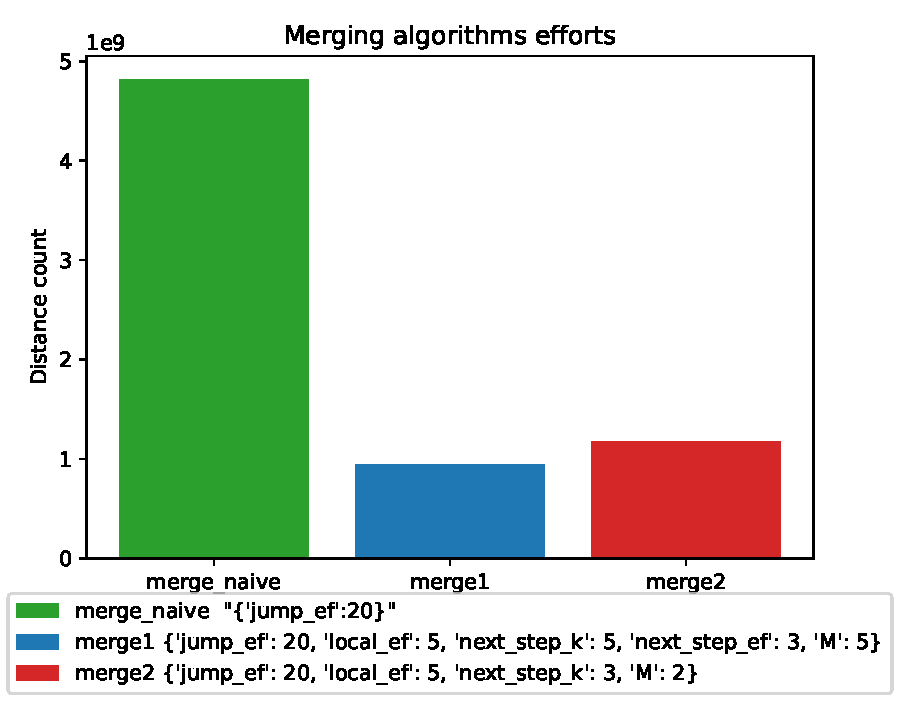
\includegraphics[width=1.\linewidth]{figs/merge-effort-comparison.pdf}
  \caption{Merging efforts}
  \label{fig:sfig1}
\end{subfigure}%
\begin{subfigure}{.5\textwidth}
  \centering
  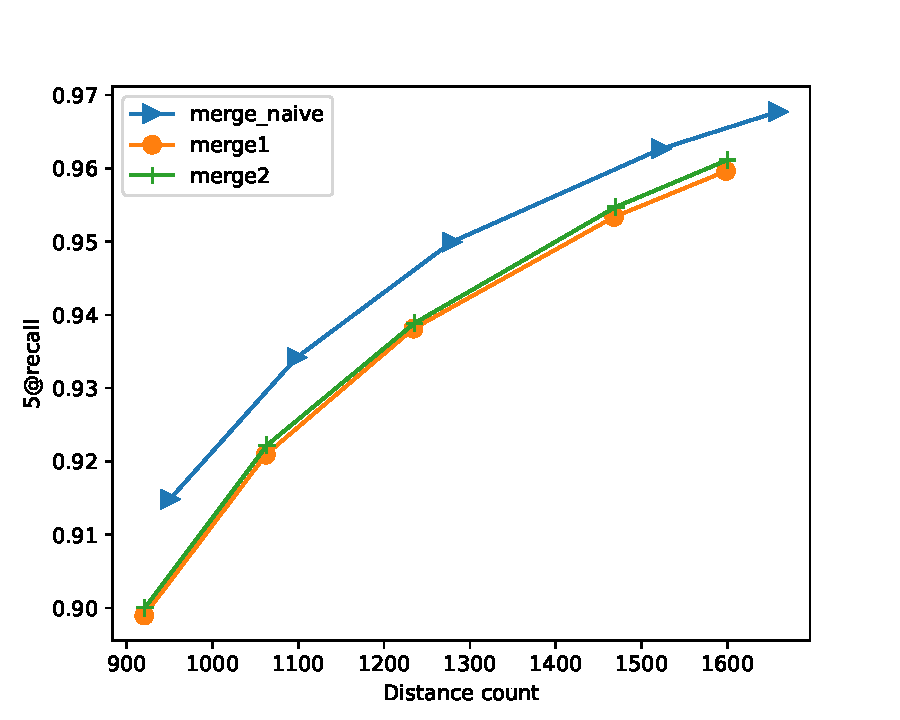
\includegraphics[width=1.\linewidth]{figs/recall-comparsion.pdf}
  \caption{Recall/computation trade off}
  \label{fig:sfig2}
\end{subfigure}
\caption{Merging algorithm comparison}
\label{fig:fig}
\end{figure}




\bibliographystyle{plain}
\bibliography{references}
\end{document}
